\documentclass[12pt]{article}
\usepackage[a4paper,margin=1in]{geometry}
\usepackage{amsmath,amssymb}
\usepackage{graphicx}
\usepackage{siunitx}
\sisetup{per-mode=symbol}
\usepackage{gvv}

\title{Matrix 4.4.11}
\author{ai25btech11015 -- M Sai Rithik}
\date{}

\begin{document}
\maketitle

\section*{Question}
The line segment joining the points \(A(2,1)\) and \(B(5,-8)\) is trisected at the points \(P\) and \(Q\), where \(P\) is nearer to \(A\). If \(P\) lies on the line
\[
2x - y + k = 0,
\]
find the value of \(k\). Use matrix / linear-algebra concepts only.

\section*{Solution}

Write the position vectors of the points using column matrices:
\begin{equation}
\Vec{A} = \myvec{2 \\ 1}, \qquad \Vec{B} = \myvec{5 \\ -8}.
\label{eq:AB}
\end{equation}

The vector from \(A\) to \(B\) is
\begin{equation}
\Vec{B}-\Vec{A} = \myvec{5 \\ -8} - \myvec{2 \\ 1} = \myvec{3 \\ -9}.
\label{eq:BA}
\end{equation}

Trisecting the segment \(AB\) means the first trisection point \(P\) (closer to \(A\)) is obtained by moving one third of the way from \(A\) toward \(B\). In vector form
\begin{equation}
\Vec{P} = \Vec{A} + \tfrac{1}{3}(\Vec{B}-\Vec{A}).
\label{eq:Pdef}
\end{equation}

Substitute \eqref{eq:AB} and \eqref{eq:BA} into \eqref{eq:Pdef}:
\begin{equation}
\Vec{P} = \myvec{2 \\ 1} + \tfrac{1}{3}\myvec{3 \\ -9}
= \myvec{2 \\ 1} + \myvec{1 \\ -3}
= \myvec{3 \\ -2}.
\label{eq:Pcoord}
\end{equation}

Thus the co-ordinates of \(P\) are \( (3, -2)\). Since \(P\) lies on the line \(2x - y + k = 0\), substitute \(x=3,\; y=-2\) into the line equation:
\begin{equation}
2(3) - (-2) + k = 0.
\label{eq:plug}
\end{equation}

Solve \eqref{eq:plug} for \(k\):
\begin{equation}
6 + 2 + k = 0 \quad\Longrightarrow\quad k = -8.
\label{eq:kval}
\end{equation}

\section*{Final Answer}
\begin{equation}
\boxed{k = -8}
\end{equation}
 \begin{figure}[h!]
    \centering
    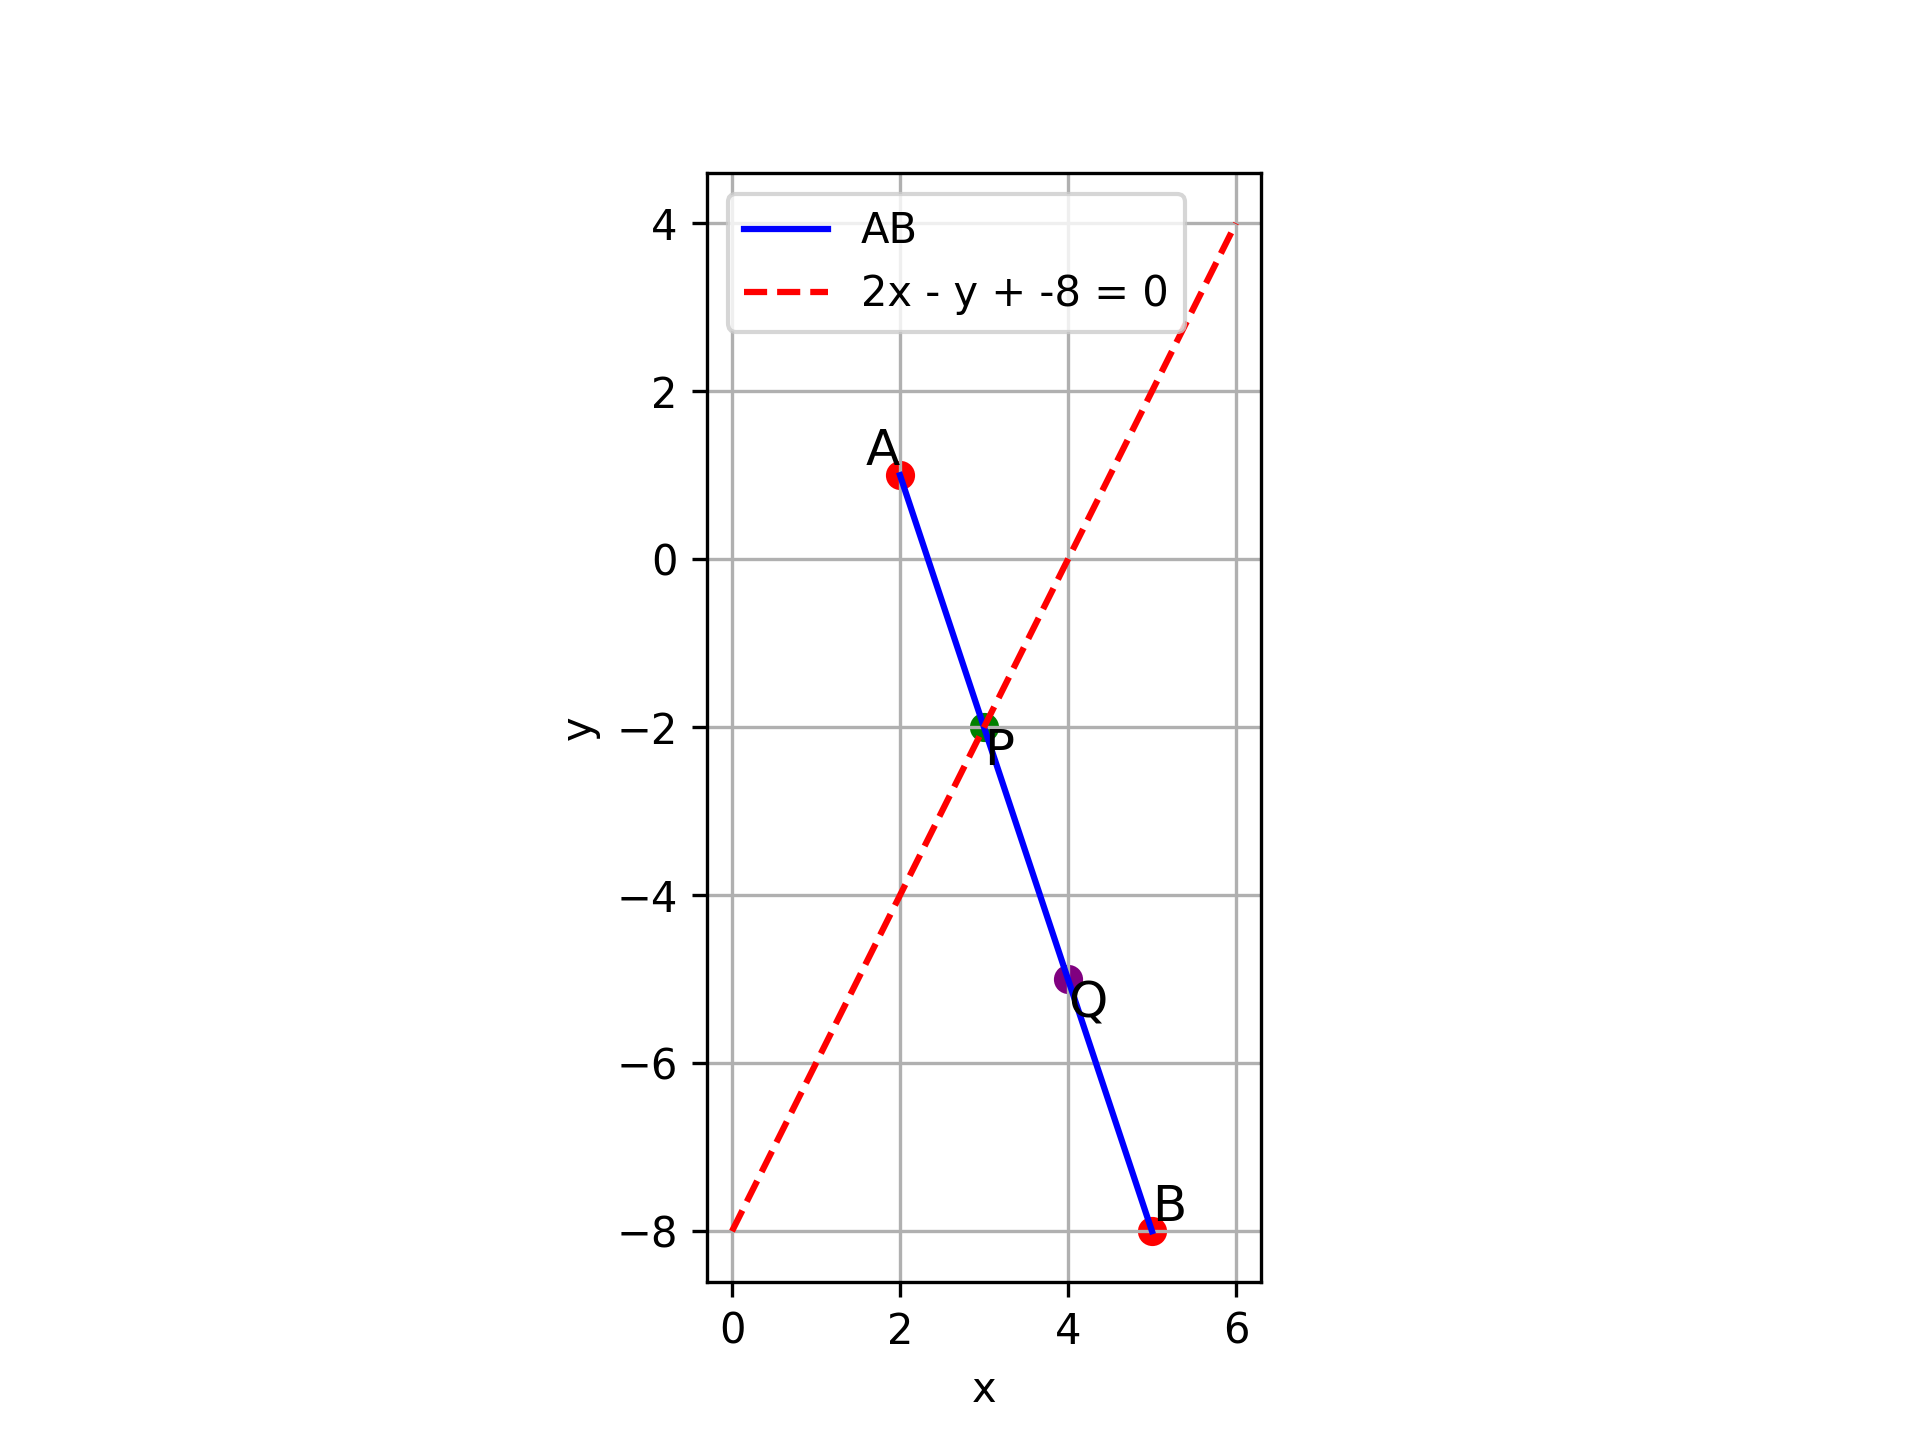
\includegraphics[width=0.65\linewidth]{figs/fig.png}
    \caption{}
\end{figure}

\end{document}
